%!TEX root=../main.tex
\chapter{Data \& Preprocessing}
\label{chap:dataset}

\section{Data Sources}

This work uses publicly available \ac{AIS} data from two geographic domains to ensure diversity in traffic patterns, waterway types, and vessel behaviours. The German datasets cover measurement stations at Kiel and Bremerhaven, recorded by \ac{AIS} receivers operated by the Bundesamt für Seeschifffahrt und Hydrographie (BSH) as part of their ship emissions monitoring programme. These data are organised by measurement station and month, downloadable per day, and publicly accessible via GovData. The U.S. dataset is sourced from the NOAA Marine Cadastre Nationwide \ac{AIS} dataset, distributed as daily CSV files covering all U.S. coastal and inland waters, and accessible via the Marine Cadastre vessel traffic portal. Records are filtered geographically to the Upper Mississippi River area within the relevant bounding box. \todo{polygon}
\subsection{Raw Data Format}

The German \ac{AIS} data are stored as semicolon-delimited log files with fields including navigation status, heading, speed (in knots with unit suffix, e.g., \texttt{6.5kt}), latitude/longitude (with hemisphere suffix, e.g., \texttt{54.419327N}), course over ground (COG), true heading, and a compact UTC timestamp (YYMMDD HHMMSS). The NOAA Marine Cadastre \ac{AIS} data follow a standardised CSV format as defined by the NOAA data dictionary, with columns \texttt{MMSI}, \texttt{BaseDateTime}, \texttt{LAT}, \texttt{LON}, \texttt{SOG}, \texttt{COG}, \texttt{Heading}, and optional vessel metadata including \texttt{VesselName}, \texttt{IMO}, \texttt{VesselType}, \texttt{Length}, \texttt{Width}, \texttt{Draft}, and \texttt{Cargo} \cite{noaa2025aisdict}.\todo{weird citation format, can I switch to [NOAA25]??}

Both datasets add unique identifiers to vessels, allowing individual tracking. 

\section{Data Preprocessing}
This section follows the structure of my implementation and refers to the files     \texttt{01\_extract.py},  \texttt{02\_clean.py}, \texttt{03\_sample.py}, \texttt{04\_track\_segmentation.py}, and \texttt{05\_normalize.py}


The raw \ac{AIS} data undergo a five-step pipeline  to produce model-ready trajectories: (1) extraction to unified CSV, (2) cleaning and filtering, (3) resampling, (4) track segmentation, and (5) normalization with feature engineering. The five steps are explained in the following:

\subsection{Extracting}

Both sources are parsed into a csv with the following core fields:

\begin{table}[ht]%output in 01_raw
\centering
\begin{tabular}{lll}
\toprule
Field & Type & Description \\
\midrule
\texttt{dataset} & string & Source identifier (e.g., \texttt{kiel}, \texttt{marinecadastre}) \\
\texttt{t\_utc} & datetime & UTC timestamp \\
\texttt{vessel\_id} & int & (hash of) MMSI number \\
\texttt{lat, long} & float & coordinates \\ %this means we can only publish the normalized data or we have to add some shift, but that is not my concern now
\texttt{sog} & float & Speed over ground (knots) \\
\texttt{cog} & float & Course over ground (degrees) \\
\texttt{heading} & float & Gyrocompass heading (degrees) \\
\texttt{rot} & float & Rate of turn ($^\circ$/min; reserved) \\
%\texttt{dt} & float & Seconds since previous update \\ not here yet
\bottomrule
\end{tabular}
\caption{Unified AIS data format after preprocessing.}
\label{tab:unified-format}
\end{table}

Additionally, dataset-specific optional fields are retained where available: \texttt{nav\_status} and \texttt{true\_heading} for the German datasets; \texttt{vessel\_name}, \texttt{imo}, \texttt{call\_sign}, \texttt{vessel\_type}, \texttt{length}, \texttt{width}, \texttt{draft}, and \texttt{cargo} for the Marine Cadastre data. 


As per ~\cite{itu-r-m1371-1-2001}, raw \ac{AIS} log files contain multiple message types beyond vessel position reports, including static and voyage-related data (Type 5), static data reports (Type 24), base station reports (Type 4), and aids-to-navigation reports (Type 21). Navigation aids (buoys etc., MMSI starting with 99) and aircrafts are filtered out. Only message types carrying dynamic position information are retained: Type 1 (Class A, scheduled), Type 2 (Class A, assigned), Type 3 (Class A, response), Type 18 (Class B), and Type 27 (long-range). These provide SOG, COG, heading, and coordinates. All other types are discarded prior to parsing. The trimmed data constitute approximately 15\% of the raw German datasets.

We fix known encoding errors, by means such as adding constant value of 102.4 to all negative SOGs and converting a heading of 511 to NaN.

\subsection{Cleaning and Filtering}

\subsubsection{Kinematic Outlier Detection:} To identify erroneous coordinates and "GPS jumps," the distance between consecutive points is calculated. If a point’s displacement exceeds what is physically achievable based on its reported Speed Over Ground (SOG) and the time elapsed since the previous timestamp, the point is discarded. During this cleaning phase, no interpolation is performed to fill the resulting gaps; this prevents the introduction of synthetic data before the formal resampling stage. Additionally, a hard threshold is applied to filter out unrealistic velocity readings, with records of any vessel reporting an SOG greater than 30 knots being excluded.

The data is further refined by applying geographic boundaries specific to each target region. These bounding boxes serve two purposes: they act as a secondary filter for large coordinate errors and allow for the subsetting of the Marine Cadastre dataset, originally provided for a much larger area, to the specific study region of the Upper Mississippi River. The defined boundaries for each dataset are detailed in Table \ref{tab:geo-bounds}:

\begin{table}[ht]
\centering
\begin{tabular}{ll}
\toprule
Dataset & Bounding Box \\
\midrule
Bremerhaven & lat $50^\circ$--$60^\circ$N, lon $5^\circ$--$10^\circ$E \\
Kiel & lat $50^\circ$--$62^\circ$N, lon $8^\circ$--$12^\circ$E \\
Marine Cadastre & lat $28.8^\circ$--$35.2^\circ$N, lon $91.0^\circ$--$88.8^\circ$W \todo{polygon} \\
\bottomrule
\end{tabular}
\caption{Initial geographic filters (02\_clean.py).}
\label{tab:geo-bounds}
\end{table}

%if this is behind table, fine. otherwise i need some new subsubsection title


Geographic coordinates are projected to UTM with the UTM zone determined automatically from the median longitude of each dataset. This Cartesian representation (metres Easting/Northing) enables accurate linear operations for resampling and normalization and allow Euclidean distance computations in loss functions. Duplicates occur when multiple stations receive the same signal: approximately two-thirds of duplicates  (same timestamp and vessel ID) are exact matches and discarded; one-third retain the row with least zero entries as first and the oldest as second criteria.

Vessel IDs have been anonymised using a one-way SHA-256 hashing function on the MMSI.
\subsection{Sampling}
\subsubsection{AIS Reporting Requirements}

The reporting frequency of \ac{AIS} transponders is non-uniform, as transmission intervals are dynamically adjusted based on vessel class, speed, and maneuvering status according to \cite{itu-r-m1371-1-2001}. Class A transponders, mandatory for large commercial vessels (typically $>300$,GT international or $>500$,GT domestic), transmit significantly more often than the Class B transponders used by smaller or recreational craft. These variable intervals, summarized in Table \ref{tab:ais-frequencies}, necessitate a standardized resampling approach to ensure temporal consistency across datasets.

\begin{table}[ht]
\centering
\begin{tabular}{lll}
\toprule
\multicolumn{3}{c}{\textbf{Class A (cargo ships, tankers, etc.)}} \\
\cmidrule(lr){1-3}
Speed/Condition & & Interval \\
\midrule
At anchor/moored, SOG $\le 3$ kn & & 3 min \\
At anchor/moored, SOG $>$ 3 kn & & 10 s \\
0--14 knots & & 10 s \\
0--14 knots + changing course & & $3\frac{1}{3}$ s \\
14--23 knots & & 6 s \\
14--23 knots + changing course & & 2 s \\
$>$ 23 knots & & 2 s \\
\midrule
\multicolumn{3}{c}{\textbf{Class B (smaller/recreational)}} \\
\cmidrule(lr){1-3}
Speed & & Interval \\
\midrule
$\le 2$ knots & & 3 min \\
2--14 knots & & 30 s \\
14--23 knots & & 15 s \\
$>$ 23 knots & & 5 s \\
\bottomrule
\end{tabular}
\caption{AIS reporting frequencies per ITU-R M.1371-01.}
\label{tab:ais-frequencies}
\end{table}
%wenn lücke zu lang, zb wegen filter oder wegen schlechten daten, leaving area ... dann split up
\subsubsection{Sampling and Interpolating}
To facilitate time-series analysis, the raw \ac{AIS} data is resampled to a uniform temporal grid. Because the NOAA Marine Cadastre data is provided at a reduced temporal resolution of 60s \cite{noaa2025aisdict}, we differentiate our processing pipeline by dataset source: the German \ac{AIS} data is interpolated to a 10s interval, whereas the Marine Cadastre data is standardized to a 60s interval.

The interpolation methodology varies by feature type. We apply linear interpolation for most telemetry features; however, geographic coordinates are interpolated using third-order splines. This ensures trajectory smoothness and more accurately reflects realistic vessel motion compared to piecewise linear paths.
After resampling, we compute the distance of each point to the closest original point for later use as a feature that indicates quality of our datapoint.

To quantify the reliability of these interpolated values, we compute a temporal offset feature, denoted as $\Delta t$. This feature represents the absolute time difference between each resampled point and its nearest original observation:
\begin{equation}
\Delta t = |t_{resampled} - t_{original, nearest}|
\end{equation}
By including $\Delta t$ as a feature in subsequent modeling steps, the system can account for interpolation uncertainty; a higher $\Delta t$ indicates a larger temporal gap in the raw data, signaling lower confidence in the precision of the interpolated state at that specific timestamp.

\subsection{Trajectory Segmentation}
This stage of the pipeline transforms cleaned vessel streams into samples suitable for trajectory prediction. By employing a sliding window approach, we maximize the utility of the available data while ensuring the physical and temporal consistency of each sample.

\subsubsection{Windowing and Stride logic}
Trajectories are partitioned into samples using a sliding window consisting of a 10-minute context window and a 2-minute prediction horizon. To ensure diversity in the dataset while managing computational redundancy, a 2-minute stride is applied between consecutive samples.To maintain the integrity of the motion dynamics, a "Time Gap Guard" is implemented: if a window spans a data blackout where the elapsed time exceeds the theoretical duration ($T_{ctx} + T_{pred}$) by more than 50\%, the segment is discarded. This ensures that the model only learns from continuous, high-fidelity motion sequences rather than fragmented data.

\subsubsection{Kinematic Filtering}
To focus the model on active vessel dynamics rather than stationary behavior, a two-tier speed filter is applied to every generated track. A track is excluded if it meets either of the following criteria:

\textbf{Anchoring Detection}: The maximum Speed Over Ground (SOG) within the segment does not exceed 1.0 knot.

\textbf{Low-Speed Persistence}: More than 30\% of the data points within the segment report an SOG below 2.0 knots.

While these filters remove a significant portion of the raw data, they are essential for isolating maneuvering patterns and preventing the model from being biased toward stationary or moored vessels.


\subsubsection{Train-Validation-Test Splitting}

To ensure robust evaluation and prevent data leakage, the dataset is partitioned at the vessel level rather than the track level. If the data were split randomly by track ID, the sliding window stride would cause the model to see overlapping temporal segments of the same vessel across the training and test sets.

Instead, unique vessel IDs are shuffled and assigned to training (60\%), validation (20\%), and testing (20\%) subsets. This ensures that the model is evaluated on its ability to generalize to entirely unseen vessels, as detailed in the methodology chapter (Section \ref{todo:methodology}).


\subsection{Feature Engineering and Normalization}
The final stage of the preprocessing pipeline involves the generation of derived motion features and the statistical standardization of the input vector. These steps are critical for ensuring numerical stability and proper gradient propagation during the model training phase.

\subsubsection{Feature Transformation}
To improve the learning of motion patterns, the raw \ac{AIS} attributes are transformed as follows:
\begin{itemize}
    \item \textbf{Relative Displacements:} Absolute UTM coordinates are converted into step-wise displacements ($dx, dy$) by calculating the difference between successive timestamps within each track ID.
    \item \textbf{Circular Encoding:} To resolve the continuity issue of the Course Over Ground (COG) at the $0^\circ/360^\circ$ boundary, the angle is decomposed into its sine and cosine components. This ensures that the periodic nature of the vessel's heading is preserved in a continuous Cartesian space.
    \item \textbf{Temporal Delta:} The $\Delta t$ feature (previously defined) is included to provide the model with context regarding the temporal reliability of the interpolated points.
\end{itemize} \todo{hier quellen wer das noch so macht einfügen}

\subsubsection{Standardization and Leakage Prevention}
We apply Z-score normalization to the feature set, transforming each variable to have zero mean and unit variance. To maintain the integrity of the experimental setup and prevent data leakage, the normalization parameters (mean $\mu$ and standard deviation $\sigma$) are computed strictly from the training partition. This global scaler is then saved and applied to the validation and test partitions without further modification. This ensures that the evaluation metrics reflect the model's performance on data drawn from a distribution established solely by the training observations.


\section{Dataset Dynamics}
\todo{hier meine plots, mit Tim absprechen was die Dynamik wirklich einfängt}

On a typical day, the Kiel and Bremerhaven datasets contain between 200 and 500 unique vessels. In contrast, the raw NOAA Marine Cadastre dataset captures approximately 15,000 vessels daily across all U.S. coastal and inland waters. Following the application of the spatial filter for the Upper Mississippi River bounding box, this volume is reduced to a highly focused subset of \todo{[insert filtered vessel count]} active inland vessels. 
Preprocessing the Kiel dataset yields approximately 1,400 trajectories per day. In total, the final model was trained across \todo{[insert total number]} datasets.

To contextualize the raw data quality prior to resampling, Figure \ref{fig:points-per-window} illustrates the distribution of \ac{AIS} messages received per vessel across various time windows (1, 5, 10, and 20 minutes) for a sample day. Figure \ref{fig:interval-hist} complements this by showing the distribution of inter-message intervals across the respective datasets, highlighting the natural reporting variability that necessitates the interpolation steps described previously. Finally, Figure \ref{fig:sample-trajectory} provides a spatial visualization of the preprocessed trajectories within the Kiel dataset, generated using \texttt{visualize.py}.



\begin{figure}[ht]
\centering
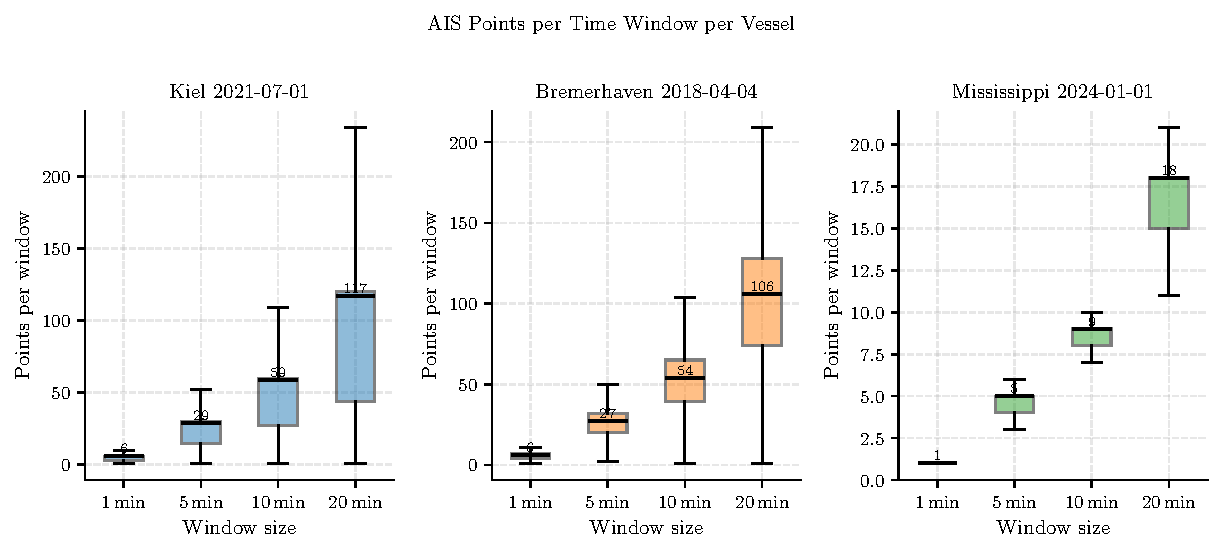
\includegraphics[width=1\textwidth]{figures/points_per_window.pdf}
\caption{Boxplot of AIS points per time window per vessel (sample day per dataset).}
\label{fig:points-per-window}
\end{figure}



\begin{figure}[ht]
\centering
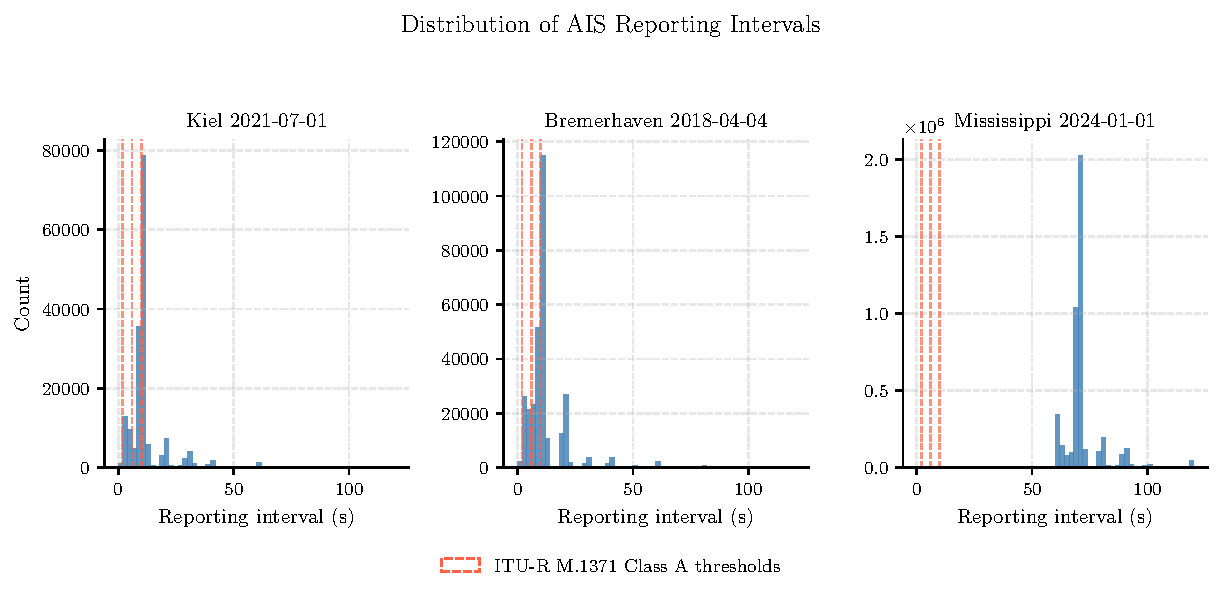
\includegraphics[width=1\textwidth]{figures/interval_hist.pdf}
\caption{Boxplot of inter-message intervals by velocity class.}
\label{fig:interval-hist}
\end{figure}

\begin{figure}[ht]
\centering
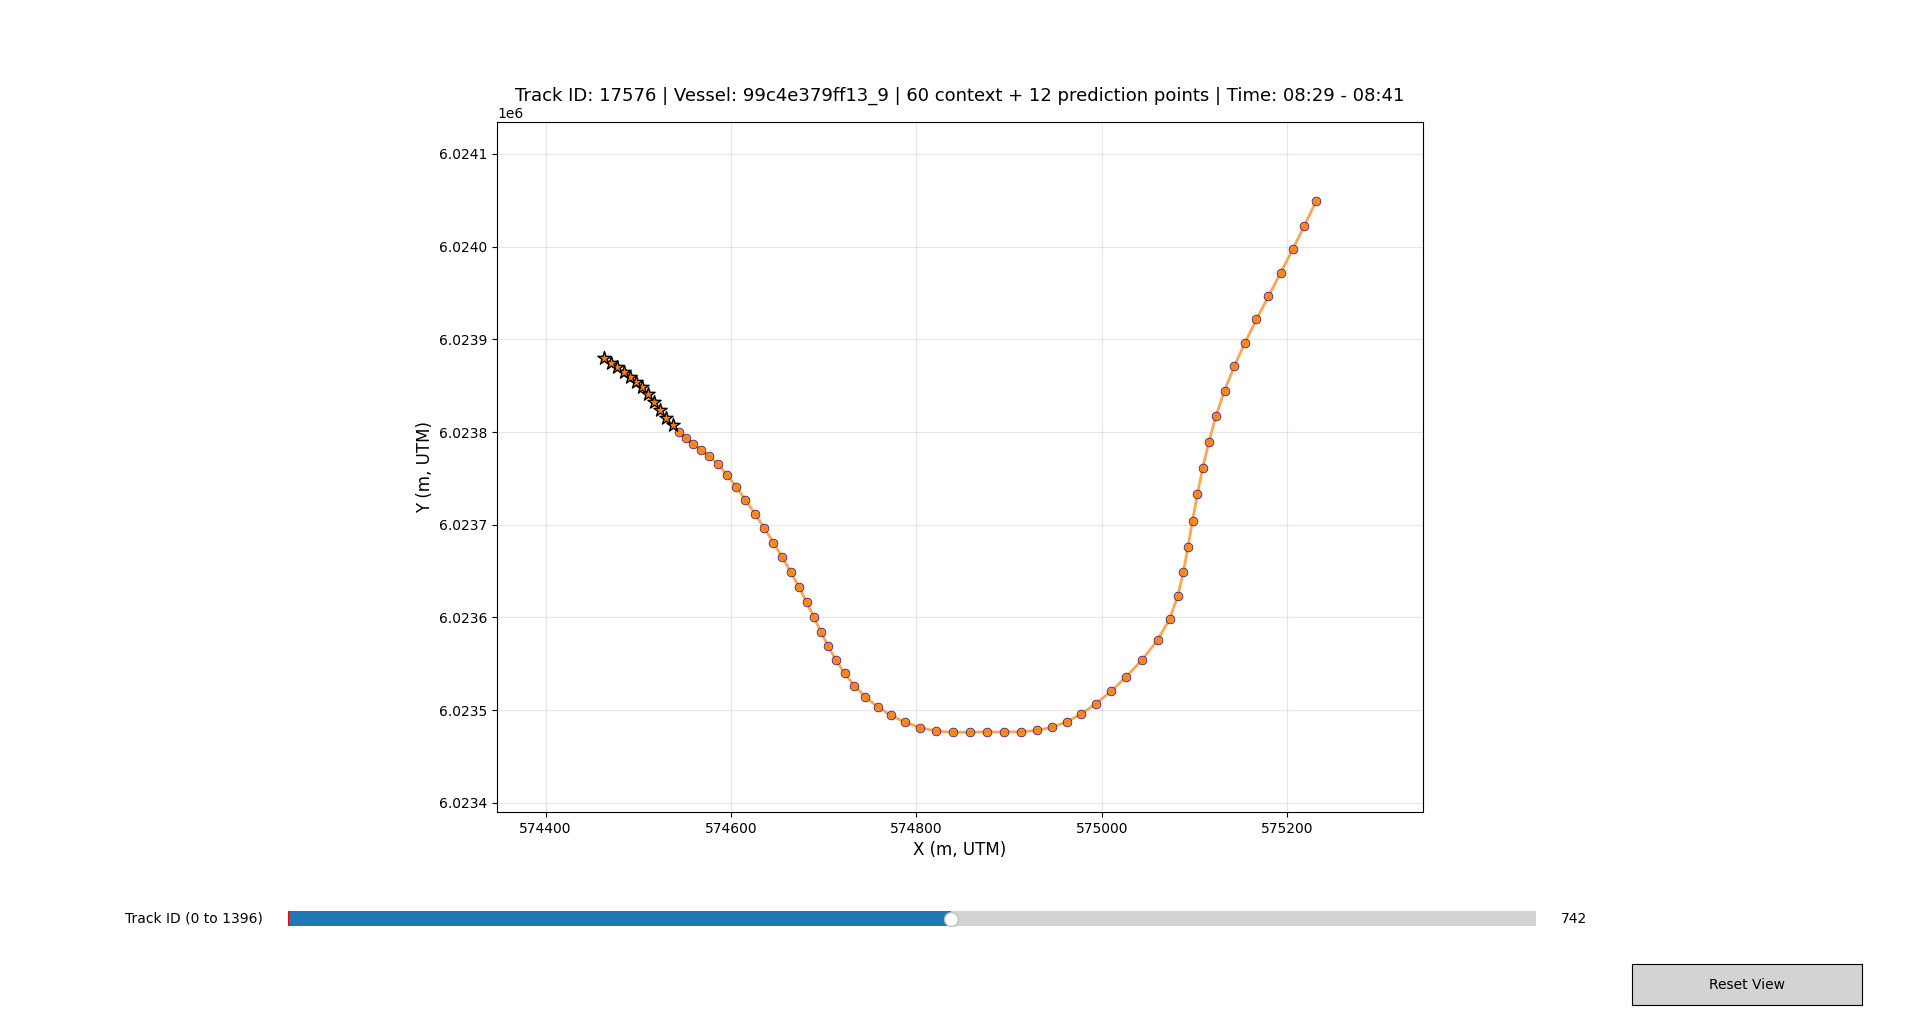
\includegraphics[width=1\textwidth, trim={9cm 3cm 9cm 2cm}, clip]{figures/kiel_trajectories_1.png}
\caption{Example training trajectory of Kiel Dataset. Circles depict Context, Stars Predictions}
\label{fig:sample-trajectory}
\end{figure}

\section{Limitations}
Despite the high fidelity of the processed datasets, several inherent limitations of the AIS system and the specific data sources must be acknowledged:
\subsubsection{Regulatory Reporting Bias}
The data primarily reflects the movement patterns of large commercial vessels mandated to carry Class A transponders under the International Convention for the Safety of Life at Sea (SOLAS) \cite{solas2014}. This includes cargo vessels exceeding 300,GT on international voyages and all tankers. Consequently, smaller recreational craft and fishing vessels utilizing Class B transponders are significantly underrepresented. Because Class B devices transmit at lower power and with less frequent update rates (as detailed in Section \ref{tab:ais-frequencies}), the resulting models may exhibit a bias toward the predictable, high-inertia dynamics of large commercial ships.


\subsubsection{Temporal Resolution and Information Loss}
The decision to use the NOAA Marine Cadastre dataset introduces a specific temporal constraint. While raw \ac{AIS} signals can be received at intervals as short as 2 seconds for fast-moving or maneuvering vessels, the NOAA archives are decimated to a fixed 60-second resolution to manage data volume \cite{noaa2025aisdict}. This reduction in sampling frequency creates a discrepancy between the German datasets (interpolated to 10,s) and the U.S. data. In high-speed scenarios or tight maneuvers, a 60-second interval may fail to capture the peak curvature of a trajectory, potentially leading to smoothing artifacts in the spline interpolation.

\todo{more? sensor noise? cheap sensors? note done if noticed in other literature}
\todo{Context labeling?}
